

\section{The Optimization Barrier of Outcome Supervision for Latent CoT}

\label{sec:optimization_barrier}

\begin{figure*}[t]
    \centering
    % --- Subfigure A: Training Dynamics ---
    \begin{subfigure}[b]{0.32\textwidth}
        \centering
        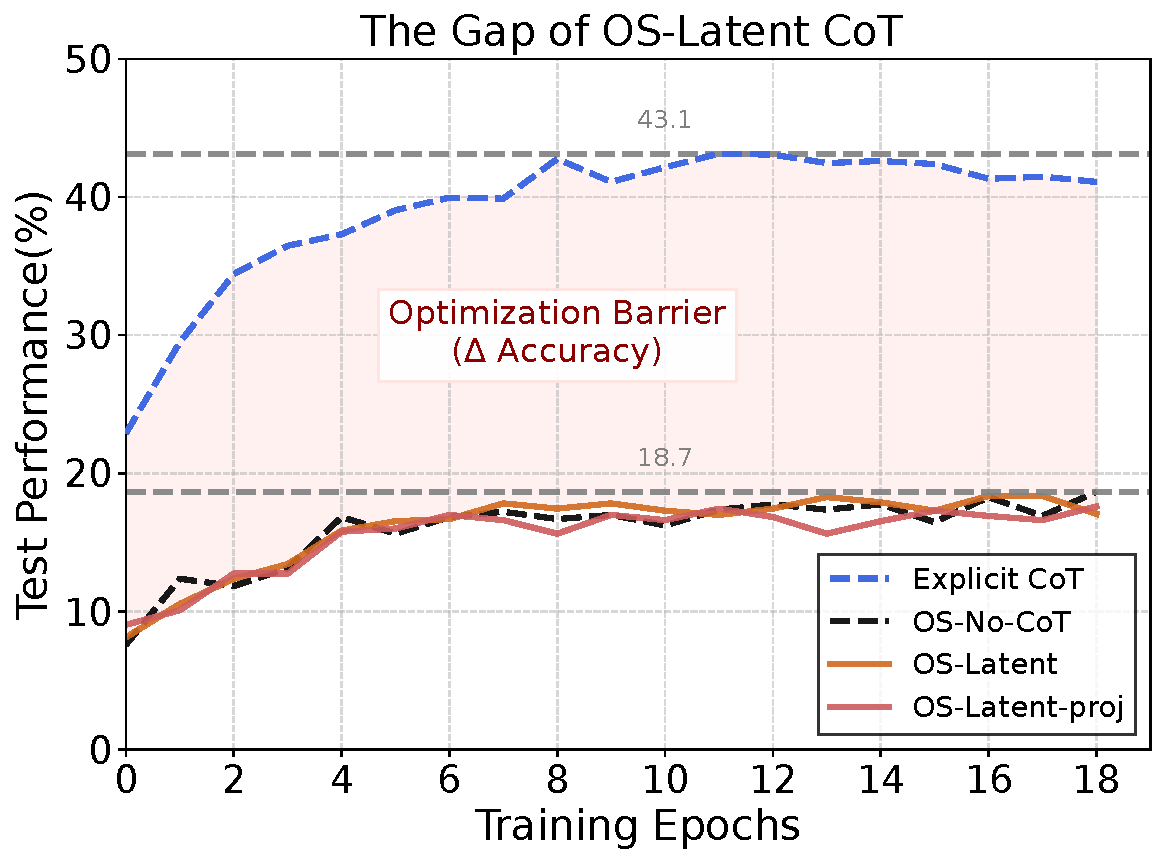
\includegraphics[width=\linewidth]{Figures/Fig1/The_Gap.pdf}
        \caption{Performance Gap}
        \label{fig:barrier_dynamics}
    \end{subfigure}
    \hfill 
    % --- Subfigure B: PCA Visualization ---
    \begin{subfigure}[b]{0.32\textwidth}
        \centering
        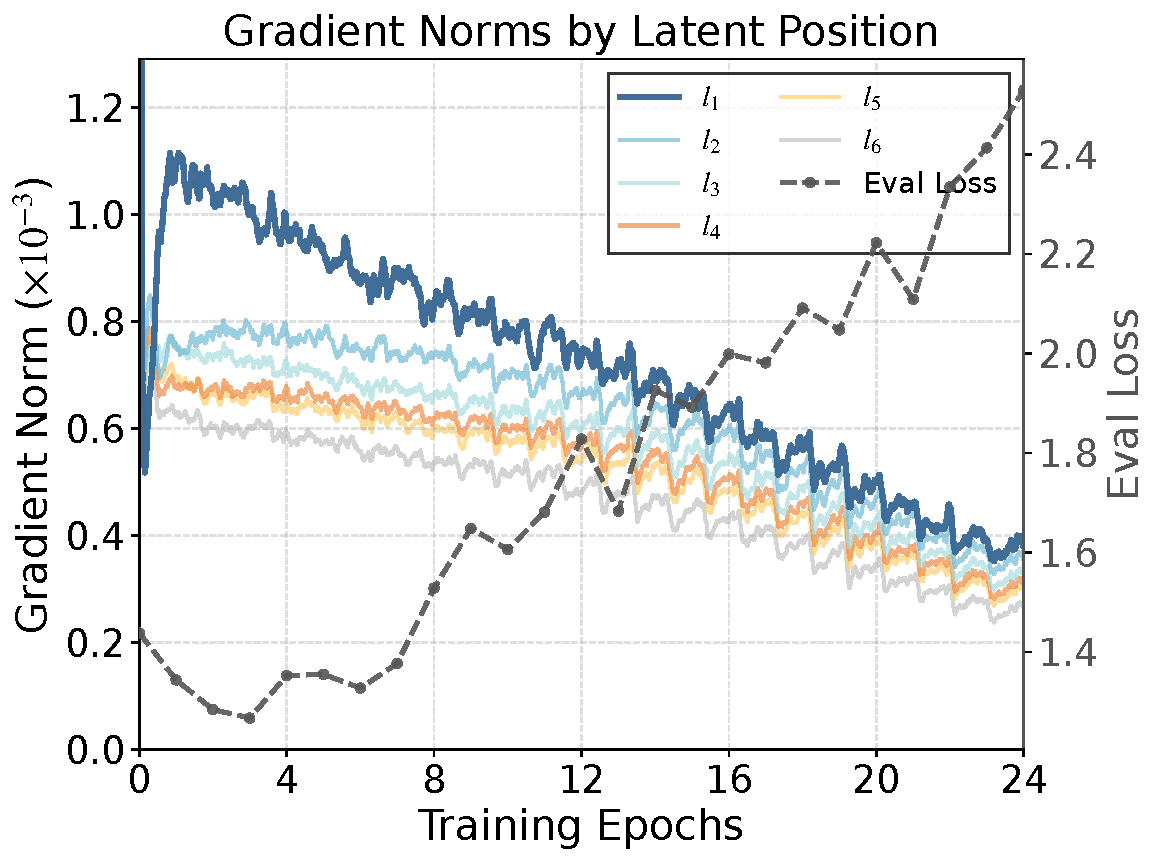
\includegraphics[width=\linewidth]{Figures/Fig1/gradient_norms_latent.pdf} 
        \caption{Gradient Attenuation}
        \label{fig:barrier_grad}
    \end{subfigure}
    \hfill
    % --- Subfigure C: Gradient Analysis ---
    \begin{subfigure}[b]{0.32\textwidth}
        \centering
        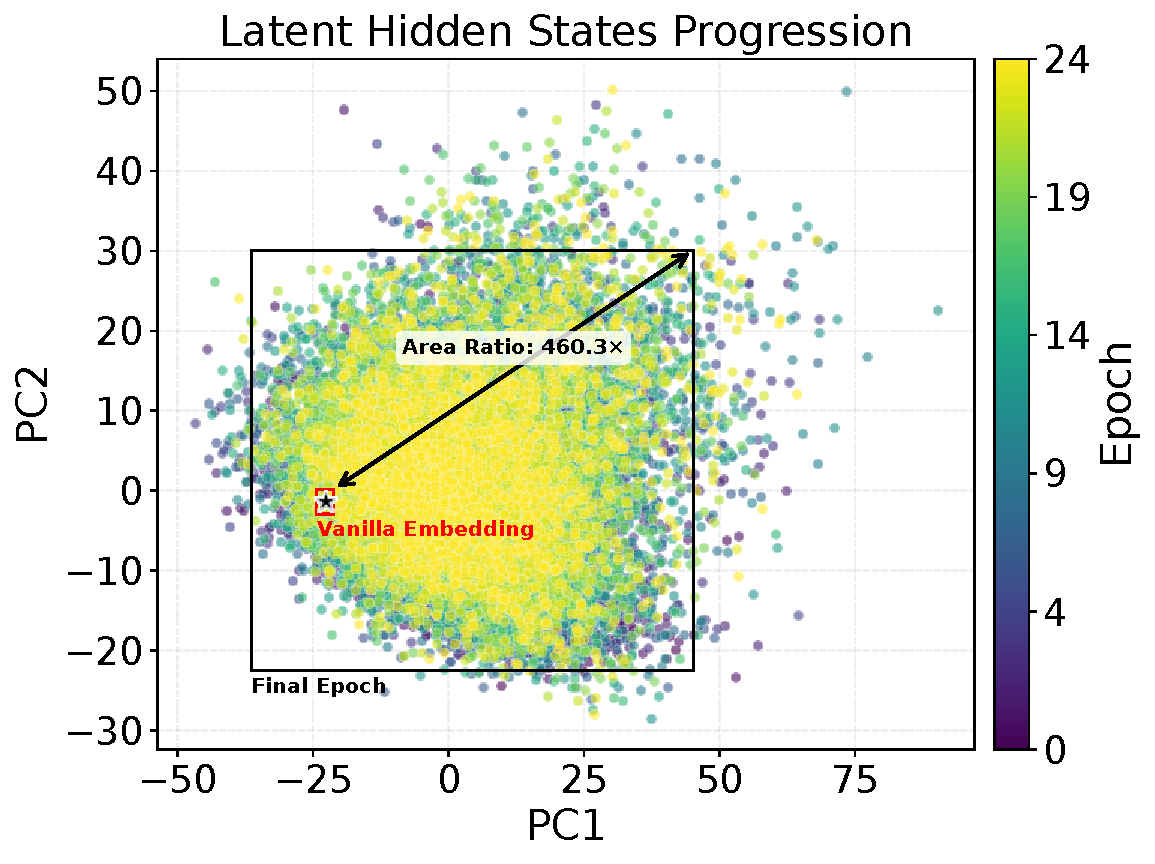
\includegraphics[width=\linewidth]{Figures/Fig1/pca_latent_evolution.pdf} 
        \caption{Manifold Drift}
        \label{fig:barrier_pca}
    \end{subfigure}
    \caption{Optimization barrier of outcome supervision.
    (a) \textbf{Performance Gap:} Despite sufficient data, all OS variants fail to bridge the gap to the explicit CoT.
    (\textbf{b}) \textbf{Gradient Analysis:} The answer-level supervision signal is unevenly distributed across latent positions, with later latent states receiving weaker gradients.
    (\textbf{c}) \textbf{Manifold Drift:} PCA visualization of OS-Latent average last-layer hidden states across training epochs. }
    \label{fig:optimization_barrier}
\end{figure*}


Prior work suggests that given sufficient data scale, Transformers can implicitly internalize multi-hop reasoning structures from input-output pairs alone~\citep{yao-etal-2025-language-models}.
This observation naturally extends to the design of Latent CoT: since continuous hidden states effectively provide additional computational depth, it is intuitively plausible that minimizing outcome loss alone should automatically pressure the model to utilize this capacity for reasoning.

Based on this intuition, we formulate the baseline hypothesis for latent CoT induction:
\textit{Given a sufficiently capable backbone and large-scale data, task-relevant latent dynamics should emerge solely from outcome supervision.}
To rigorously test this, following prior work~\citep{hao2025training}, we employ a GPT-2~\citep{radford2019language} backbone trained on the augmented GSM8k~\citep{cobbe2021trainingverifierssolvemath} dataset (GSM8k-Aug, ~\citealt{deng2023implicitchainthoughtreasoning}). We minimize the standard negative log-likelihood over the final answer $y$:
\begin{equation}
    \mathcal{L}_{\mathrm{OS}} = - \frac{1}{|y|} \sum_{i=1}^{|y|} \log p_{\theta}(y_i \mid x, L, y_{<i}),
\end{equation}

where the continuous hidden states are implicitly integrated into the forward pass of the backbone (See Appendix~\ref{app:hyper} and~\ref{app:os_ps_pseudocode} for detailed configurations).


\paragraph{The Collapse of Outcome-Supervised Latent CoT.}
\label{subsec:collapse_observation}
We compare the training trajectories of Explicit CoT (Upper Bound) against a suite of Outcome-Supervised baselines.
As shown in Figure~\ref{fig:barrier_dynamics} and Table~\ref{tab:part1}, the Explicit CoT steadily converges to viable performance level, indicating that the backbone has sufficient parameter capacity to solve these multi-step reasoning tasks when provided with explicit intermediate steps.
In contrast, removing this intermediate supervision leads to a substantial performance drop~\footnote{We include additional generalization experiments in Appendix~\ref{app:os_generalization}.}. Both \textsc{OS-Latent} and \textsc{OS-Latent-proj} \emph{fail to outperform} the trivial \textsc{OS-No-CoT} baseline. 
To understand why it fails to improve performance, we analyze the underlying optimization dynamics that govern the evolution of the continuous hidden states:


\paragraph{Gradient Attenuation.}
To diagnose the mechanistic cause of this collapse, we analyze the gradient flow dynamics governing the latent chain. We quantify the supervision magnitude reaching each step $t$ via the gradient norm $\mathcal{G}(t)$:
\begin{equation}
% \mathcal{G}(t) = \left\| \frac{\partial \mathcal{L}}{\partial h_{t-1}} \right\|_2
\mathcal{G}(t) = \left\| \frac{\partial \mathcal{L}_{\mathrm{OS}}}{\partial L_t} \right\|_2
\label{eq:grad_norm}
\end{equation}
Figure~\ref{fig:barrier_grad} reveals a position-wise gradient attenuation. The supervision signal is concentrated on $L_1$, while $L_{2\dots6}$ suffers from systematic signal loss, effectively flattening into inactivity.
The resulting dynamics show an early-improvement-then-degradation pattern. The validation loss decreases primarily during the initial phase when early latent states receive stronger gradients. As these gradients decay, the loss stops improving and eventually rebounds, indicating that later latent states do not receive sufficient supervision to assume the reasoning burden. This behavior is consistent with a structural shortcut: instead of distributing computation across the latent trajectory, the model relies disproportionately on early latent positions to support the final prediction. This resembles gradient starvation~\citep{pezeshki2021gradient}, where dominant shallow features suppress the learning of deeper dependencies.

\paragraph{Manifold Drift.}
This structural bypass leads to an unstable evolution of the latent space.
Figure~\ref{fig:barrier_pca} visualizes the PCA trajectory of the OS-Latent hidden states across training epochs, referenced against the static semantic space of Explicit CoT embeddings.
The continuous hidden states exhibit significant manifold drift: since the intermediate latent states are only indirectly constrained by the final-answer loss, they lose their semantic tethering. Instead of moving toward stable semantic anchors, the trajectory diverges into an unstructured region.
This confirms a fundamental geometric disconnect: without active participation in the gradient flow to constrain the search space, the optimization process fails to keep the intermediate representations close to the semantic reference region induced by explicit CoT embeddings.

This analysis explains the Optimization Barrier: gradient short-circuiting precipitates manifold drift, showing that outcome supervision provides only a weak and distal surrogate for increasing the answer-level mutual information $I(L;y)$, without ensuring that individual latent states preserve valid reasoning information.

